Consid\'erons un r\'eseau \'electrique mod\'elis\'e  par un DAG et une matrice $\mu_c$ dans laquelle chaque ligne/colonne est associ\'ee \`a un arc du DAG.
Une case de $\mu_c[i,j]$ contient le niveau de corr\'elation de mesures entre l'arc $i$ et l'arc $j$, une valeur entre $0$ et $1$. Toutefois des erreurs de mesures peuvent apparaitre.
\newline
Id\'ealement, si ces deux arcs partagent une extr\'emit\'e en commun, soit l'extr\'emit\'e initiale ou soit l'extr\'emit\'e finale comme dans la figure \ref{typeSommetsEnCommun}, la valeur est proche de $1$ sinon elle est proche de $0$.
	\begin{centering}\vspace{-0.5em}
	\begin{figure}[htb!]\vspace{-0.5em}
	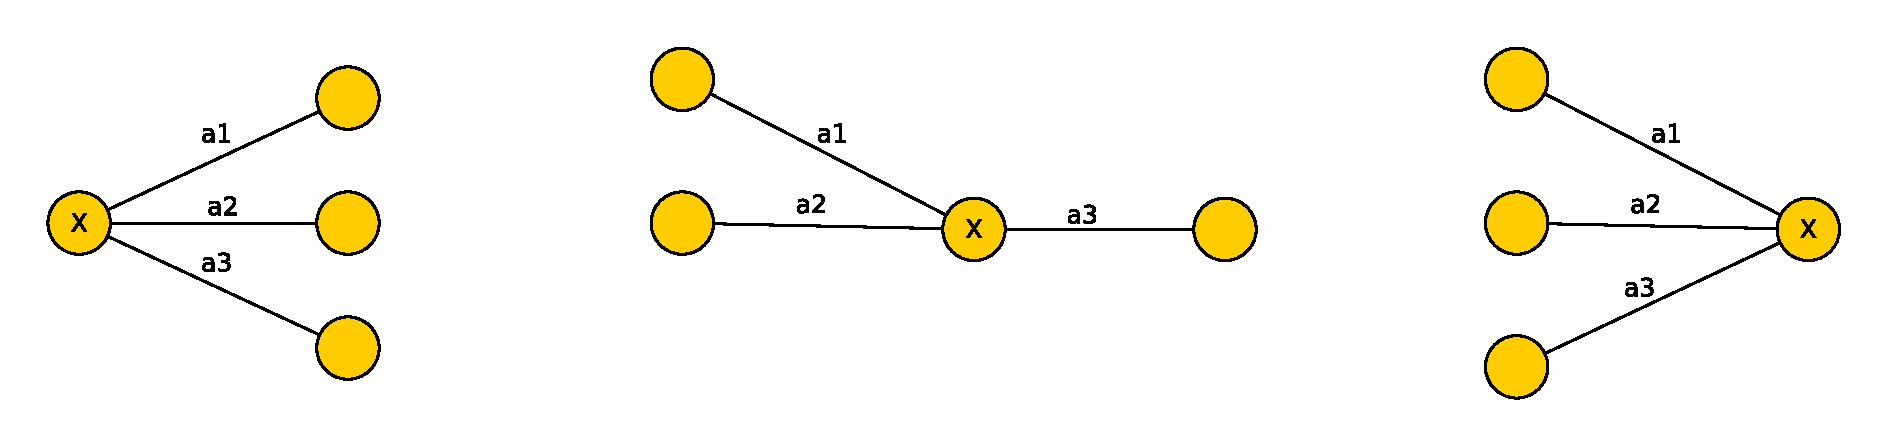
\includegraphics[scale=0.50]{typeSommetsEnCommun.eps}\vspace{-0.5em}
	\caption{ Sommet $X$ partag\'e entre les ar\^etes. De la gauche vers la droite : sommet entrant, \`a droite sommet interm\'ediaire et sommet sortant }\vspace{-0.5em}
	\label{typeSommetsEnCommun}
	\end{figure}
	\end{centering}
\`A partir de $\mu_c$ et d'une valeur de seuil choisie $s \in [0,1]$, on consid\`ere la matrice $M$ de m\^eme dimension que $\mu_{c}$ dans laquelle 
$M[i,j] = 1$ ssi $\mu_c[i,j] \ge s$, sinon $M[i,j] = 0$. 
\newline
Soit $G_C = (V_C,E_C)$ le graphe dont $M$ est la matrice d'adjacence.
Id\'ealement, l'ensemble des liens ayant une extremit\'e commune forme une clique dans $G_C$.

\begin{definition}
	Un graphe $G_C = (V_C, E_C)$ est un graphe de corr\'elation ssi il est le line graphe d'un DAG.
	L'ensemble $\cal C$ est dit une {\bf couverture de corr\'elation} de $G_C$
\end{definition}

\subsubsection{D\'etermination du graphe de corr\'elation et sa line-couverture}
	\begin{definition}
	Une ambiguit\'e est un graphe isomorphe \`a l'un des graphes de la figure \ref{configurationAmbiguite}. Le sommet $X$ est appel\'e le {\bf point d'ambiguit\'e}.
	\end{definition}
	
	\begin{centering}\vspace{-0.5em}
	\begin{figure}[htb!]\vspace{-0.5em}
	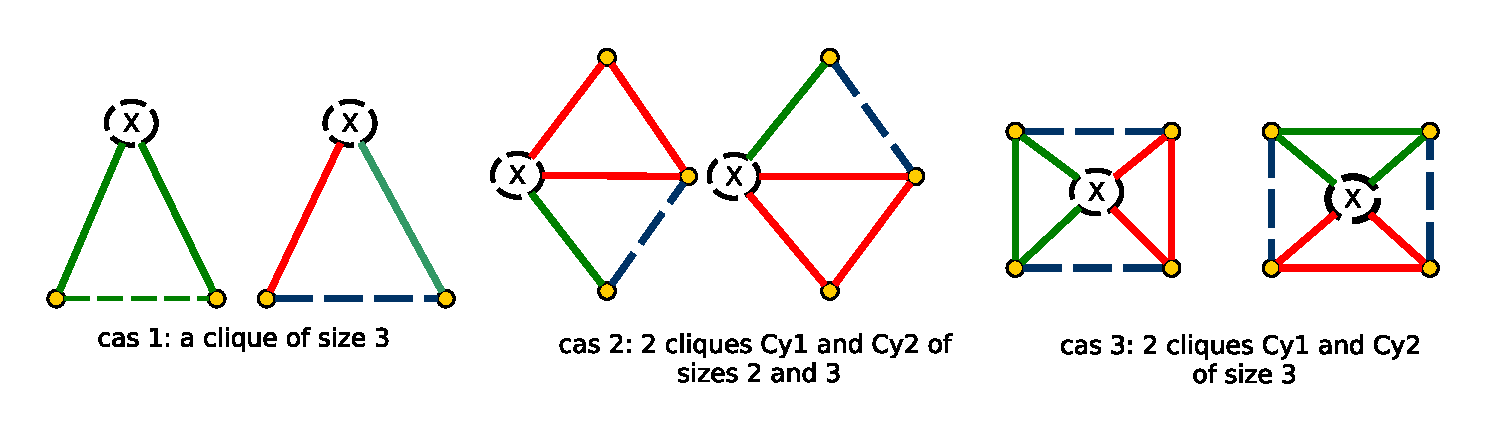
\includegraphics[scale=0.70]{configurationAmbiguite.eps}\vspace{-0.5em}
	\caption{ Configurations possibles d'une ambiguit\'e au sommet X }\vspace{-0.5em}
	\label{configurationAmbiguite}
	\end{figure}
	\end{centering}
	
	\begin{lemma}
	Si un graphe de corr\'elation $G_C$ admet deux couvertures de corr\'elation, alors il existe au moins un sommet $u$ de $G_C$ tel que $G_{C}[\{u\} \cup \Gamma_{G_C}(u)]$ est une ambiguit\'e dont $u$ est le point.
	\end{lemma}
	
	\begin{proof} 
		Consid\'erons deux line-couvertures $C$ et $C'$ de $G_C$. 
		Il existe au moins un sommet $v \in G_C[V]$ qui n'est pas couvert par la (ou les) m\^eme(s) clique(s) dans $C$ and $C'$.
		Soient deux cliques $c_1$ et $c_2$ (potentiellement vide) partitionant $\{v\} \cup \Gamma_{G_C}(v)$ dans $\cal C$.
		Consid\'erons deux autres cliques $c_3$ et $c_4$ diff\'erentes de $c_1$ et $c_2$partitionant \'egalement $\{v\} \cup \Gamma_{G_C}(v)$ dans $\cal C$. \newline
		Notons $c_{i,j}$ l'intersection de $c_{i}$ et $c_j$ pour tout $i \in \{1,2\}$ et $j \in \{3,4\}$. 
		Chaque sommet $w \in c_{i,j}$ est couvert par au plus deux cliques de $G$ dans $\cal C$, dont la clique $c_i$.
		Puisque $c_j$ est une clique alors ce sommet $w$ est voisin de tous les sommets de  $c_{i',j}$, pour $i' \ne i$.
		Les ar\^etes entre ces sommets sont dans $c'_i$, donc chaque ar\^ete $[w,z]$ pour tout sommet  $z \in c_{i',j}$ forme une clique correspondant dans le r\'eseau de flots.
		Ainsi, le cardinal de chaque ensemble  $c_{i,j}$ est \'egal \`a $1$.\newline
		Appelons $v_{i,j}$ le seul sommet pr\'esent dans $c_{i,j}$. 
		Il est possible d'avoir $v_{1,3} = v_{1,4}$ ou $v_{2,3} = v_{2,4}$.
		Si les deux \'egalit\'es sont v\'erifi\'ees, le sommet $v$ \'est alors couvert non pas par deux cliques mais par une seule de cardinalit\'e $3$.
		Ainsi, les seuls cas possibles sont alors r\'esum\'es par la figure  \ref{graphe2Couverture}.
		Le sommet $v$ est bien le point d'une ambiguit\'e isomorphe \`a $G_C[\{u\} \cup \Gamma_{G_C}(u)]$.
	\end{proof}

On peut d\'eduire le corollaire suivant :
\begin{corollary}
Si un graphe de corr\'elation admet deux couvertures de corr\'elation, alors il est isomorphe \`a l'un des graphes de la figure  \ref{graphe2Couverture}.
\end{corollary}
\begin{centering} \vspace{-0.5em}
\begin{figure}[htb!] \vspace{-0.5em}
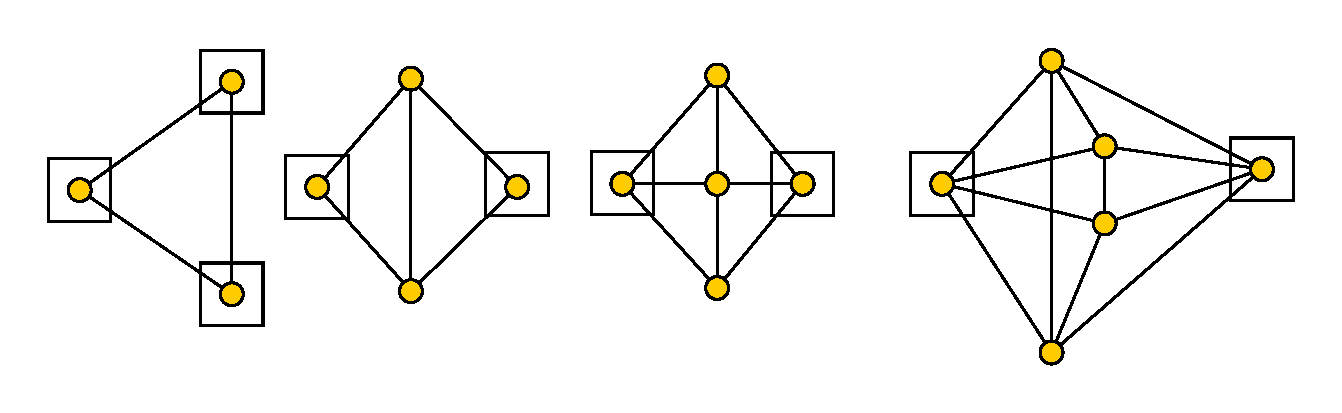
\includegraphics[scale=0.75]{graphe2Couverture.eps}
\caption{ Graphes possibles avec deux couvertures avec les points d'ambiguit\'es }
\label{graphe2Couverture} 
\end{figure}
\end{centering} 
En Effet, si $G_C[{u} \cup \Gamma_{G_C}(u)]$ est une ambiguit\'e, chaque ar\^ete, qui n'est pas li\'ee au point d'ambiguit\'e, doit \^etre une ar\^ete d'une et une seule autre ambiguit\'e de $G_C$. Et chaque sommet d'une ambiguit\'e, qui n'est pas un point d'ambiguit\'e, doit appartenir \`a une et une seule autre ambiguit\'e de $G_C$ dont il n'est pas non  plus le point d'ambiguit\'e.
De plus, chaque ar\^ete, n'\'etant pas couvert par les deux configurations de cliques possibles dans une ambiguit\'e (les ar\^etes en pointill\'ees dans la figure \ref{graphe2Couverture}), doivent \^etre dans la m\^eme situation dans une autre ambiguit\'e \`a laquelle elles appartiennent.
Ces contraintes font que si un graphe contient une ambiguit\'e induite, alors il ne peut \^etre que dans un cas de la figure  \ref{graphe2Couverture}.

\begin{definition}
Soit $G$ un graphe et $u$ un sommet de $G$. Une partition de $\Gamma_G(v)$ en deux cliques $C_{u1}, C_{u2}$ est {\bf coh\'erente } ssi chaque sommet $v$ de $C_{u1}$ (resp $C_{u2}$) a au plus un voisin dans $C_{u2}$  (resp $C_{u1}$).
\end{definition}
Le r\'esultat suivant est un corollaire direct de la preuve du lemme \ref{lemmaCoherente}
\begin{lemma}
\label{lemmaCoherente}
Soit $G_C$ un line graphe, $u$ un sommet de $G_C$ et une partition coh\'erente de ${u} \cup \Gamma_{G_C}(v)$ en deux cliques  $C_{u1}, C_{u2}$. 
Si l'une de ces deux cliques est de cardinal sup\'erieur ou \'egal \`a $4$, alors cette partition coh\'erente est unique.
\end{lemma}

\'Etant donn\'e une partition coh\'erente $C_{u1}, C_{u2}$ pour un sommet $u$ de $G_C$, la fiabilit\'e de cette coh\'erence est
$F(C_{u1}, C_{u2}) = \min\limits_{[x,y] \in E(C_{u1} \cup E(C_{u2} )}  \mu_{C}([x,y])$

\begin{definition}
Une {\bf line-couverture} d'un graphe non orient\'e connexe $G_C$ est un ensemble de cliques maximales de $G_C$ telles que chaque sommet de $G_C$ appartient \`a une ou deux de ces cliques et que chaque ar\^ete de $G_C$ soit couverte par exactement une de ces cliques.
\end{definition}

Il a \'et\'e montr\'e qu'un graphe $G_C$ est  un line graphe si et seulement si il admet une line-couverture.
Bas\'ee sur cette id\'ee et sur des sous-graphes exclus, un algorithme lin\'eaire en fonction du nombre d'ar\^etes a \'et\'e propos\'e pour v\'erifier  si un graphe est un line graphe et si oui en fournir la line-couverture.
Cette algorithme est {\bf l'algorithme de couverture}.


